\section{Verify Result}
\label{sec:verify}

After letting the \ac{AI} run a number of iterations (100,000; 500,000; 1,000,000), we evaluated the success of the learning algorithm.

The first test was to see whether the \ac{AI} had learned the "rules" of the game. We tested this by plotting the number of invalid moves against the epsilon value: With a higher epsilon value, more random moves were made and therefore more invalid moves were to be expected.
At later stages, with more learned moves, we expected to see very few invalid moves.

The graphs below shows the development of the number of times invalid moves were made by either of the \ac{AI} players compared to the epsilon value in percent (red and green for the invalid move numbers, blue for epsilon).
In both cases the epsilon value starts at 1, meaning that only random actions are carried out and is decreased by 0.001 at each interval so that exactly 1,000 intervals are needed before only learned actions are done. In the first graph \ref{fig1}, the interval is at 150 for 500,000 games, the second \ref{fig2} shows 1,000,000 games with a 300 interval.

This means that (in theory), for the second run, the \ac{AI} had double the time to learn steps from random actions.
\begin{figure}[H]
	\centering
  	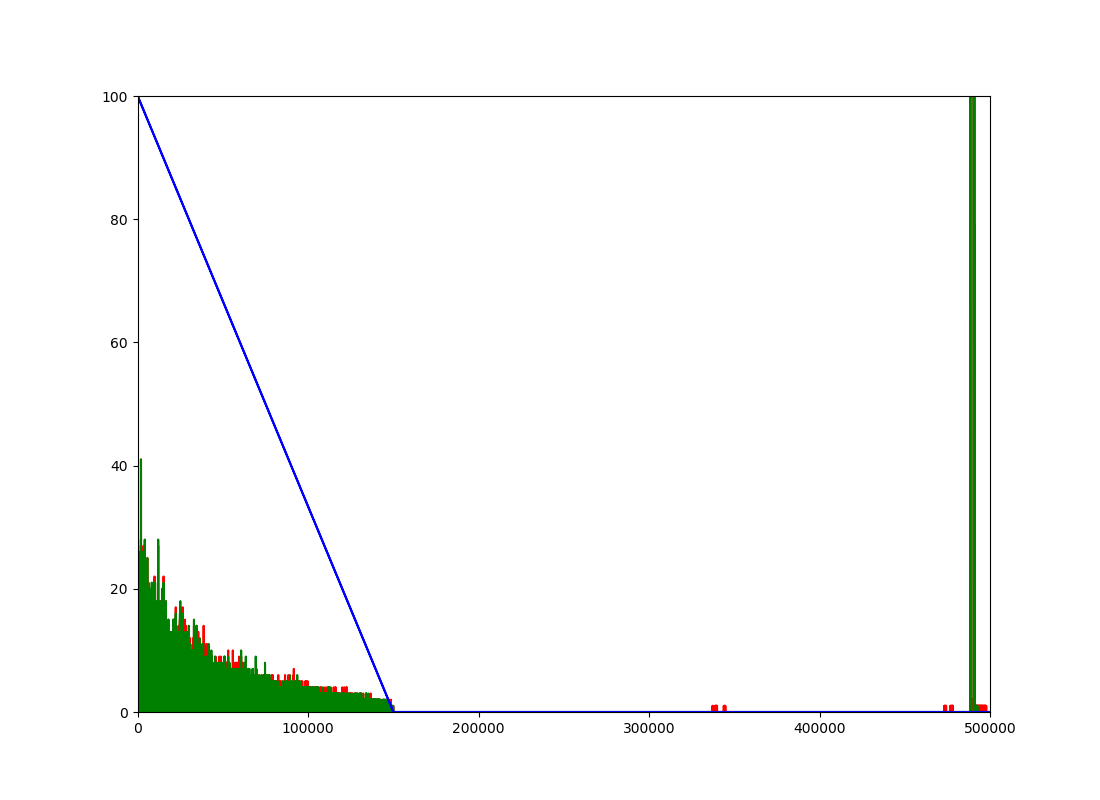
\includegraphics[width=\textwidth]{../plot_500k.png}
	\caption{500 000 iterations}
	\label{fig1}
\end{figure}

\begin{figure}[H]
	\centering
	%plot1m.png??
  	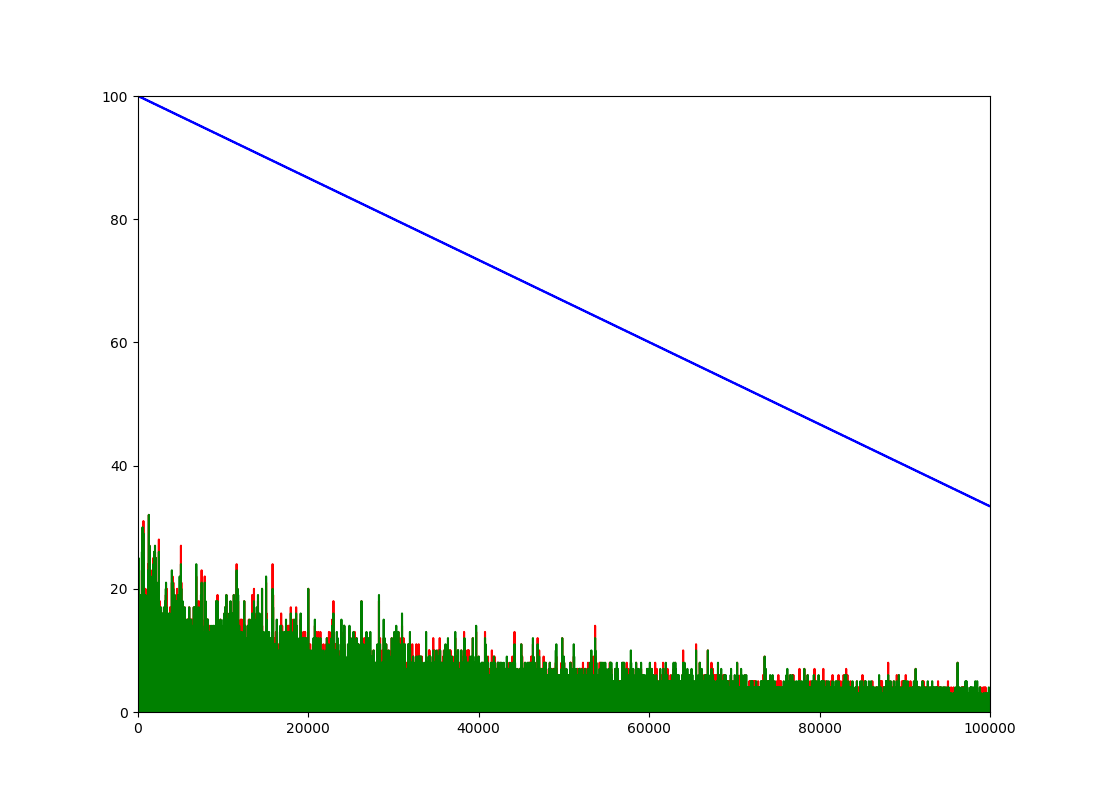
\includegraphics[width=\textwidth]{../plot_100k.png}
	\caption{100 000 iterations}
	\label{fig2}
\end{figure}

Both graphs show that the number of invalid moves declines steadily with the epsilon value, reaching effectively no invalid moves once epsilon reaches zero, except for very few outliers.

The graph\ref{fig3} below shows this transition in detail: Before the epsilon value reaches zero, invalid moves are made now and then, but afterwards none happen anymore.
\begin{figure}[H]
	\centering
  	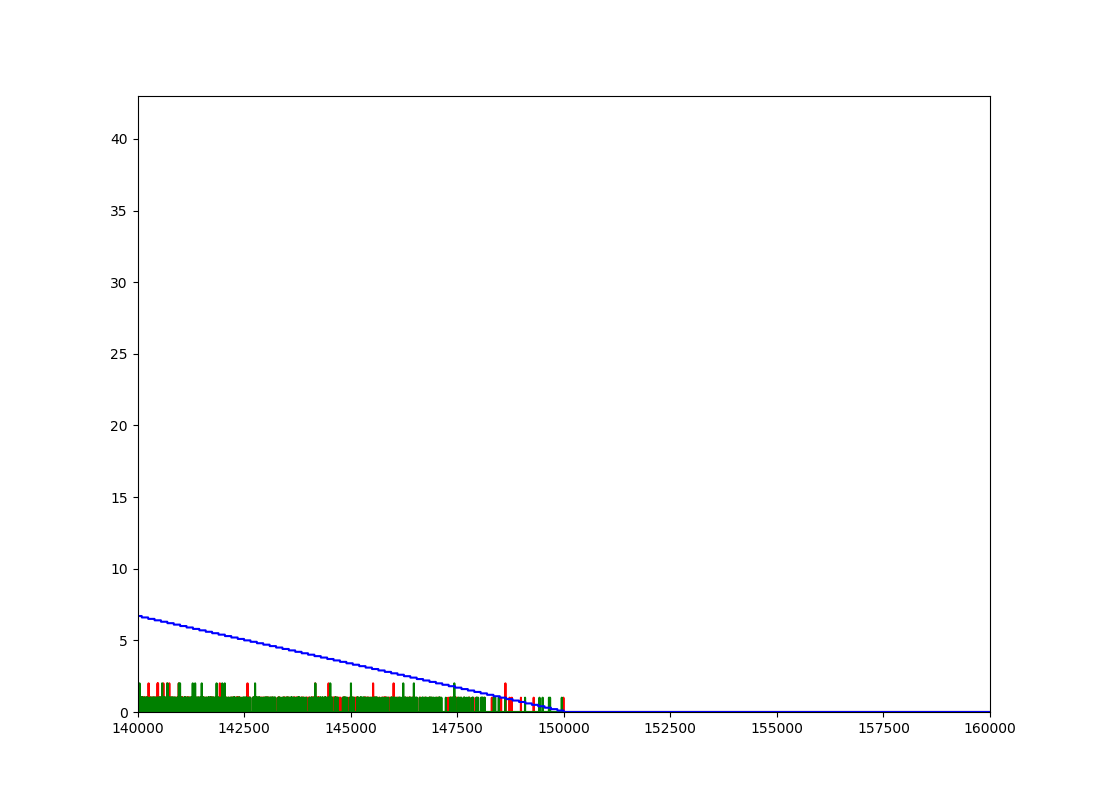
\includegraphics[width=\textwidth]{../plot_500k_transition.png}
	\caption{Transition area between the 140 000 and 160 000 iteration}
	\label{fig3}
\end{figure}

This leads us to the conclusion that the \ac{AI} models did indeed learn the rules of the game: Hardly any invalid moves were made once they were allowed to used their knowledge without forced random moves.


The second test was to let the \ac{AI} play against a human opponent: This would show us whether it only learned general rules or whether it had actually developed the ability to play tactics.

The results are shown in the following table \ref{aiGameResults}

\begin{table}[H]
	\begin{tabular}{|l|c|c|}\hline
		AI iterations & Human wins & AI wins \\ \hline \hline
		100k & 0 & 0 \\ \hline
		500k & 0 & 0 \\ \hline
		1m & 0 & 0 \\ \hline
	\end{tabular}
	\caption{AI versus human results}
	\label{aiGameResults}
\end{table}